\section{Идеи для хобби}
\begin{epigraph}
    Хобби --- это способ уйти от скуки.
\end{epigraph}

\begin{figure}[ht!]
    \centering
    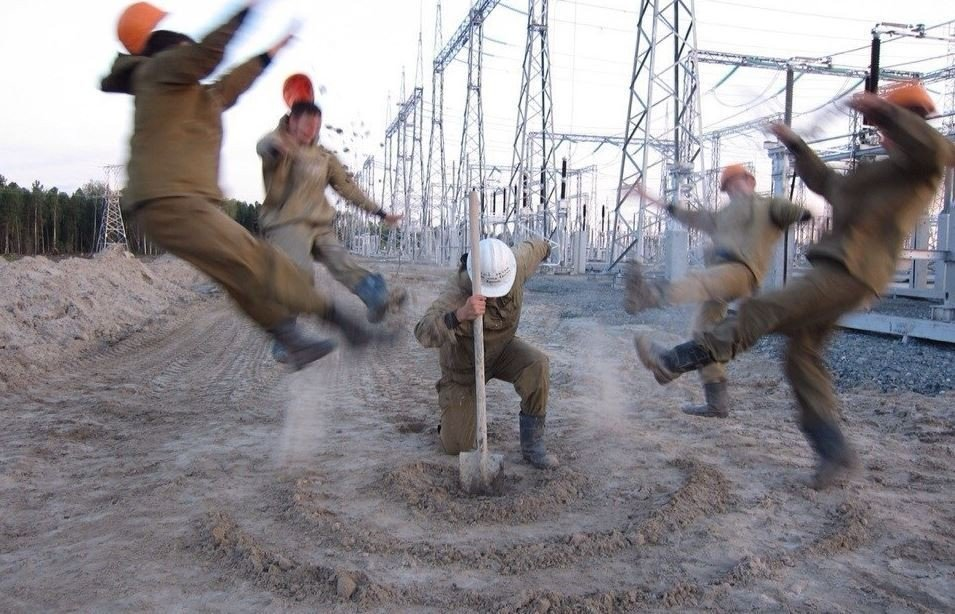
\includegraphics[width=\textwidth]{smile-please}
    \caption{not boredom, make photo}
\end{figure}

\begin{itemize}
    \item Собирать идеи для хобби
    \item Собрать библиотеку из самых странных (по содержанию, автору, оформлению и т.д.) книг из когда-либо выпущенных человечеством.
    \item Искать забавные представления занятным числам:
    \begin{itemize}
        \item  $42 = 2^5 + 2 \cdot 5$
        \item  $145 = 1! + 4! + 5!$
        \item  $1729 = 19 \cdot 91 = 1^3 + 12^3 = 9^3 + 10^3$
        \item  $22 = 16_{16}$
    \end{itemize}
    \item Придумывать скороговорки, начинающиеся/заканчивающиеся на одну букву:
    \begin{flushleft}
        \begin{verse}
        Виолончелисты ввалились в вагон,\\
        Виолончели выпали вкось.\\
        Виолончелисты вышли вон,\\
        Виолончели валяются врозь.\\

        Виолончелисты в Вирджинии вдоль\\
        Виолончели в ведро водрузили.\\
        Виолончелисты внимательно вдаль\\
        Виолончели вновь вукатили!\\

        "Вертай всё взад" - вернувшись веолончедисты все вскричат.\\
        Виолончель внутри вся влажная ---\\
        Восвояси вскорь выпроважена.
        \end{verse}
    \end{flushleft}

    \item (для ленивых) Коллекционировать прожитые годы.
    \item Искать в других языках (и придумывать новые в своём) для обозначения различных странных состояний: как, например, называется состояние, когда есть желание вернуться в то место, из которого ещё не уехал?
    \item Собирать/придумывать различные способы для изучения алфавитов.
    
    % нужно переверстать данное место в TeX
    \begin{figure}[ht!]
        \centering
        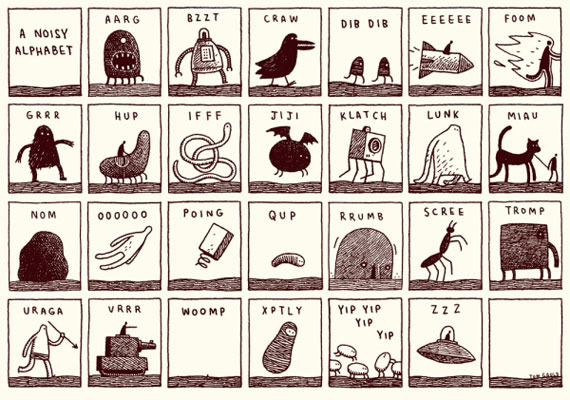
\includegraphics[width=\textwidth]{abc}
        \caption{Один из вариантов алфавита}
    \end{figure}
    
    \item телефон с экраном покрывающийся жиром (для любителей всё время протирать экран телефона)
    \item комната автоматически распрыскивающая пыль (для неугомонных поборников чистоты)
    \item кофе со вкусом: чая, лапши, плова, борща и т.д. (для истинных ценителей необычного) + можно и обратно
    \item булочка с чайной начинкой (аналог два в одном)
    \item солёный сахар и сладкая соль
    \item съедобные свечи
    \item кофе без кофеина, сигареты без никотина, алкоголь без спирта, суп без воды ... (вообще без) и бонус 'жизнь без смысла'
    \item деревянная печь/духовка/...
    \item подпольная китайская палата мер и весов
    \item переводчик на любой язык кроме нужного
    \item огурцы с молоком, пирожки с макаронами, чай с тефтелями и другие невероятные блюда
    \item кофе пресованное в кубики (как сахар)
    \item губораскатывающая машина (закатывающая же есть)
    \item решать задачки в текстовом редакторе (для садистов --- в терминале)
\end{itemize}
% просто спам
\begin{figure}[ht!]
    \centering
    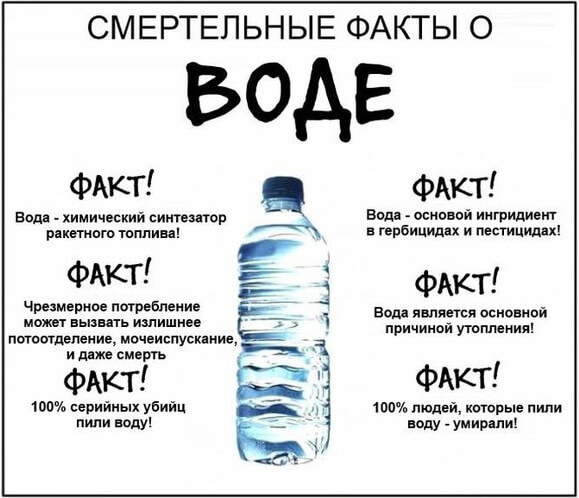
\includegraphics[width=\textwidth]{wat}
    \caption{Хватит пить! Остановись! Ещё не поздно!}
\end{figure}
